\documentclass[landscape, a4paper]{article}
\usepackage[margin=0cm,top=0.4cm,bottom=0.4cm,left=0.4cm,right=0.4cm]{geometry}
% \usepackage[showframe,margin=0cm,top=0.5cm,bottom=0.5cm,left=0.5cm,right=0.5cm]{geometry}
\usepackage[export]{adjustbox}
\usepackage{xcolor}
\usepackage{caption}
\usepackage{csquotes}
\usepackage{titlesec}
\usepackage{etoolbox} % Add this to your preamble
\usepackage[parfill]{parskip}

\newtoggle{isEnglish}
\toggletrue{isEnglish}
% \togglefalse{isEnglish}

\captionsetup{labelformat=empty, justification=centering, font={color=PrimaryColor}}

\definecolor{PrimaryColor}{HTML}{8FA85F}
\newcommand\alert[1]{\textcolor{PrimaryColor}{\textbf{#1}}}

\titleformat{\section}
{\color{PrimaryColor}\normalfont\normalsize\bfseries}
{\thesection}{0.5cm}{}
\titlespacing{\section}{0cm}{0.2cm}{0.2cm}
% \renewcommand{\thesection}{\arabic{section}}

\titleformat{\subsection}
{\color{PrimaryColor}\normalfont\normalsize\bfseries}
{\thesubsection}{0.5cm}{}
\titlespacing{\subsection}{0cm}{0.1cm}{0.1cm}

\begin{document}
\noindent
\centering
\footnotesize
\begin{minipage}[t]{0.31\textwidth}
	\setlength{\parskip}{0.25cm}

	\vspace{0.5cm}

		\textcolor{PrimaryColor}{
			\rule{\linewidth}{0.5mm}
			\vspace{-0.1cm}
			\begin{center}
				\large
        \textsc{\iftoggle{isEnglish}{Hike to the Kybfelsen castle ruin}{Wanderung zur Burgruine Kybfelsen}}
			\end{center}
			\rule{\linewidth}{0.5mm}
		}

    \iftoggle{isEnglish}{
    An unforgettable hike through the enchanting natural landscape of Freiburg's \alert{Günterstal}, up to the mysterious castle ruins of Kybfelsen! The path leads deep into the forest, past babbling brooks, imposing rocks, and magical clearings. After just a few steps, you are immersed in the peaceful silence of the Black Forest, where you are enveloped by towering trees and swallowed by the woods, escaping the hustle and bustle of the big city.

    The \alert{Arboretum in Günterstal} invites you on a journey through the world of trees. A selection of planted trees and shrubs has been organized by theme and equipped with informational signs. Each of the five themed trails is dedicated to a region of origin, a group of related tree species, or a special aspect of the relationships between the world of trees and the world of animals or humans.
  Many of the trees here are botanical treasures, including living fossils like the ginkgo and ancient conifers that have survived since the time of the dinosaurs. With over 1,300 species, the Arboretum is one of the most diverse collections of its kind in Germany.}{
		Eine unvergessliche Wanderung durch die zauberhafte Naturlandschafft des Freiburger \alert{Günterstals} hinauf zur mysteriösen Burgruine Kybfelsen! Der Weg führt tief in die Wälder, vorbei an plätschernden Bächen, imposanten Felsen und verwunschenen Lichtungen. Schon nach den ersten Schritten taucht man in die friedvolle Stille des Schwarzwalds ein, wo man unter den mächtigen Bäumen voll und ganz vom Wald verschluckt wird und der Hektik der Großstadt entfliehen kann.

		Das \alert{Arboretum in Günterstal} lädt zu einer Reise durch die Welt der Bäume. Dafür wurde eine Auswahl der gepflanzten Bäume und Sträucher nach Themen geordnet und mit Hinweistafeln versehen. Jeder der fünf Themenpfade ist einem Herkunftsgebiet, einer Gruppe verwandter Baumarten oder einem besonderen Aspekt der Beziehungen zwischen der Lebenswelt der Bäume und der Lebenswelt der Tiere oder Menschen gewidmet.
  }
    % It also includes unique paths such as the \enquote{WaldMenschen} sculpture trail and the \enquote{Mycelium} trail, which explores the underground world of fungi and forest ecosystems.

		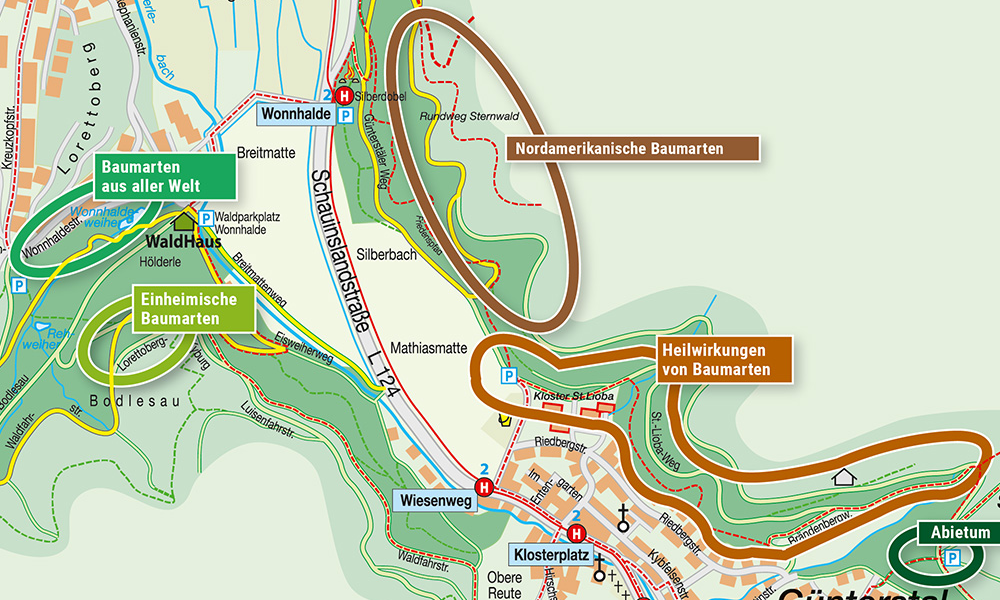
\includegraphics[width=\linewidth]{./figures/arboretum.png}
    \captionof{figure}{\iftoggle{isEnglish}{Arboretum in Günterstal with its themed trails}{Arboretum in Günterstal mit seinen Themenpfaden}}
		\setlength{\parskip}{0.25cm}

    \iftoggle{isEnglish}{
    An \alert{arboretum} (Latin, a variant of arbustum, here specifically in the sense of tree planting, from arbor meaning tree) is a collection of various, often exotic woody plants (not grown in containers). This can be, for example, a botanical garden in which primarily trees and shrubs are planted. If only shrubs are planted, it is referred to as a fruticetum. If only coniferous trees are planted in an arboretum, it is called a pinetum. In case of Firs, the corresponding term is Abietum and so on.
  }{
		Ein \alert{Arboretum} (lat.\ Nebenform zu arbustum hier speziell im Sinne von Baumpflanzung von arbor Baum) ist eine Sammlung (nicht in Pflanzgefäßen wachsender) verschiedenartiger, oft auch exotischer Gehölze; dies kann beispielsweise ein botanischer Garten sein, in dem hauptsächlich Bäume und Sträucher angepflanzt werden. Man spricht von einem Fruticetum, wenn nur Sträucher angepflanzt werden. Werden in einem Arboretum nur Nadelgehölze angepflanzt, nennt man es Pinetum.
  }

\end{minipage}%
\hfill%
\vrule width 0.01cm
\hfill%
\begin{minipage}[t]{0.31\textwidth}
	\vspace{0cm}
	\setlength{\parskip}{0.25cm}
    \iftoggle{isEnglish}{
  The \alert{Stadtwald Arboretum} was established as early as the late 19th century, when Freiburg's foresters began planting exotic tree species in nearby forests for experimental purposes. However, only a few tree species were successfully integrated into the native forest ecosystem. The most famous and characteristic example for Freiburg's Stadtwald is the forestry use of the North American tree species Douglas fir, which has been used in forestry in Freiburg since 1896 and is now one of the most economically important tree species.
}{
	Das \alert{Stadtwald-Arboretum} entstand bereits Ende des 19. Jahrhunderts, als die Freiburger Förster in stadtnahen Wäldern begannen, fremdländische Baumarten zu Versuchszwecken zu pflanzen. Jedoch gelang nur bei wenigen Baumarten die Integration in die heimische Waldgesellschaft. Das wohl berühmteste und für den Stadtwald Freiburg charakteristische Beispiel ist die forstwirtschaftliche Nutzung der nordamerikanischen Baumart Douglasie, die bereits seit 1896 in Freiburg forstwirtschaftlich genutzt wird und heute eine der wirtschaftlich wichtigsten Baumarten ist.
}

	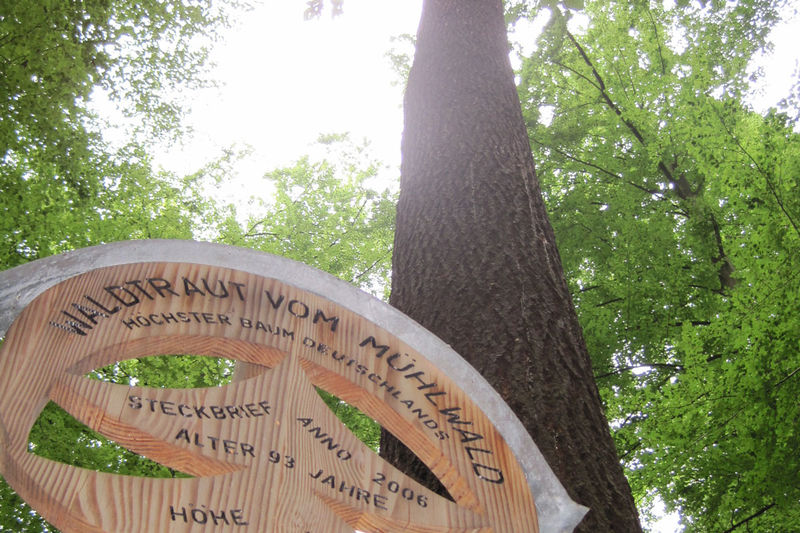
\includegraphics[width=\linewidth]{./figures/waldraud.png}
  \captionof{figure}{\iftoggle{isEnglish}{Waldtraut of the Mühlwald, the tallest officially measured tree in Germany}{Waldtraut vom Mühlwald, höchster amtlich vermessener Baum Deutschlands}}
	\setlength{\parskip}{0.25cm}

    \iftoggle{isEnglish}{
  The \alert{Douglas fir} is economically significant in the Black Forest because it grows quickly, is resistant to drought and pests, and provides high-quality wood that can be used in a variety of ways. Additionally, as part of mixed forests, it improves the stability and resilience of the forest, making it especially attractive in the face of climate change.\\
By the way, the name Douglas fir has nothing to do with the perfume and cosmetics company Douglas. The name of the Douglas fir comes from the Scottish botanist David Douglas, who brought the tree species from North America to Europe in the 19th century. The name of the company Douglas, on the other hand, goes back to the founder John Sharp Douglas, who opened a soap factory in Hamburg in 1821, which later became a perfume and cosmetics company.

  A special highlight along the route is \alert{Waldtraud}, the (in the year 2025) 115-year-old Douglas fir, which, with its proud height of 67 meters, holds the title of tallest tree in Germany. It was planted in 1913 as a three-year-old tree at its current location, slightly south of today's Arboretum in Günterstal.

However, the hiking route has even more to offer: at several viewpoints, you can enjoy breathtaking views over Freiburg and Günterstal. In addition to the landscape, you also experience a piece of history, many famous personalities have left their mark here.
}{
	Die \alert{Douglasie} ist im Schwarzwald wirtschaftlich bedeutsam, weil sie schnell wächst, robust gegenüber Trockenheit und Schädlingen ist und qualitativ hochwertiges Holz liefert, das vielseitig genutzt werden kann. Zudem verbessert sie als Teil von Mischwäldern die Stabilität und Widerstandsfähigkeit des Waldes, was sie angesichts des Klimawandels besonders attraktiv macht.\\
	Der Name Douglasie hat übrigens nichts mit dem Parfüm- und Kosmetikunternehmen Douglas zu tun. Der Name der Douglasie leitet sich vom schottischen Botaniker David Douglas ab, der die Baumart im 19. Jahrhundert aus Nordamerika nach Europa brachte. Der Name des Unternehmens Douglas hingegen geht auf den Gründer John Sharp Douglas zurück, der 1821 eine Seifenfabrik in Hamburg eröffnete, die später zu einem Parfüm- und Kosmetikunternehmen wurde.

	Ein besonderes Highlight auf der Strecke ist \alert{Waldtraud}, die (im Jahr 2024) 114 Jahre alte Douglasie trägt mit ihren stolzen 67 Metern Höhe den Titel als höchster Baum Deutschlands. Sie wurde 1913 als dreijährige Pflanze an den jetzigen Standort etwas südlich des heutigen Arboretums Freiburg-Günterstal gesetzt.

	Die Wanderroute hält allerdings noch mehr bereit: An mehreren Aussichtspunkten kannt man atemberaubende Blicke über Freiburg und das Günterstal genießen. Neben der Landschaft erlebst man auch ein Stück Geschichte, viele berühmte Persönlichkeiten haben hier ihre Spuren hinterlassen.
}

\end{minipage}%
\hfill\color{white}%
\vrule width 0.01cm
\hfill\color{black}%
\begin{minipage}[t]{0.31\textwidth}
	\vspace{0cm}
	\setlength{\parskip}{0.25cm}

    \iftoggle{isEnglish}{
  \alert{Günterstal} is mentioned by name for the first time in a deed of ownership from the year 804, at that time as \enquote{Gundherrerhusir} (houses of Günther) in the Mark of Merzhausen. Around 300 years later, the place appears again under the name \enquote{Guntheristal}. Around 1221, a nobleman, who according to an 18th-century tradition was named Günther von Kibenfels, gave the land in Günterstal to his daughter Adelheid. There, she and her companions built a small monastic complex. In a document from 1224, the monastery in \enquote{Günterstal} is mentioned for the first time. However, Günther von Kibenfels cannot be the namesake of the place, since the name \enquote{Günter} had already appeared much earlier in the place name. Along the hiking route, you also pass the gatehouse of the former monastery, which is crossed by the streetcar.

  Among others, the prominent German mathematician \alert{Ernst Zermelo} is buried in the cemetery in Günterstal in Freiburg. His grave lies next to that of Edmund Husserl. Ernst Zermelo was a significant mathematician who revolutionized set theory. He formulated the Zermelo axiom system, which forms the foundation of modern set theory. Particularly well-known are the \alert{Zermelo-Fraenkel axioms}, which precisely define the mathematical structure of sets and are widely used in mathematics today. Another important result of his work is the Axiom of Choice, which is essential in many areas of mathematics, such as analysis and algebra. Zermelo's contributions laid the foundation for many modern mathematical theories.
}{
	Namentlich erwähnt wird \alert{Günterstal} zum ersten Mal in einer Besitzurkunde aus dem Jahr 804, damals als \enquote{Gundherrerhusir} (Häuser des Günther) in der Mark von Merzhausen. Rund 300 Jahre später taucht der Ort unter dem Namen \enquote{Guntheristal} wieder auf. Um 1221 schenkt ein Adeliger, der einer Überlieferung aus dem 18. Jahrhundert zufolge Günther von Kibenfels hieß seiner Tochter Adelheid das Gelände in Günterstal. Dort baut sie mit ihren Gefährtinnen eine kleine klösterliche Anlage. In einer Urkunde von 1224 wird das Kloster in \enquote{Günterstal} erstmals erwähnt. Günther von Kibenfels kann jedoch nicht der Namensgeber des Ortes sein, da der Name \enquote{Günter} schon sehr viel früher im Ortsnamen auftauchte. Auf der Wanderroute kommt man auch am Torhaus des ehemaligen Klosters vorbei, welches von Straßenbahn durchfahen wird.

	Unter anderem ist der bedeutende deutsche Mathematiker \alert{Ernst Zermelo} auf dem Friedhof in Günterstal in Freiburg beerdigt. Sein Grab liegt neben dem von Edmund Husserl. Ernst Zermelo war ein bedeutender Mathematiker, der die Mengenlehre revolutionierte. Er formulierte das Zermelo-Axiomensystem, das die Grundlage für die moderne Mengenlehre bildet. Besonders bekannt sind die \alert{Zermelo-Fraenkel-Axiome}, welche die mathematische Struktur von Mengen präzise definieren und heute in der Mathematik weit verbreitet sind. Ein weiteres wichtiges Resultat seiner Arbeit ist das Auswahlaxiom, das in vielen Bereichen der Mathematik, wie der Analysis und Algebra unerlässlich ist. Zermelos Beiträge legten die Grundlage für viele moderne mathematische Theorien.
}

	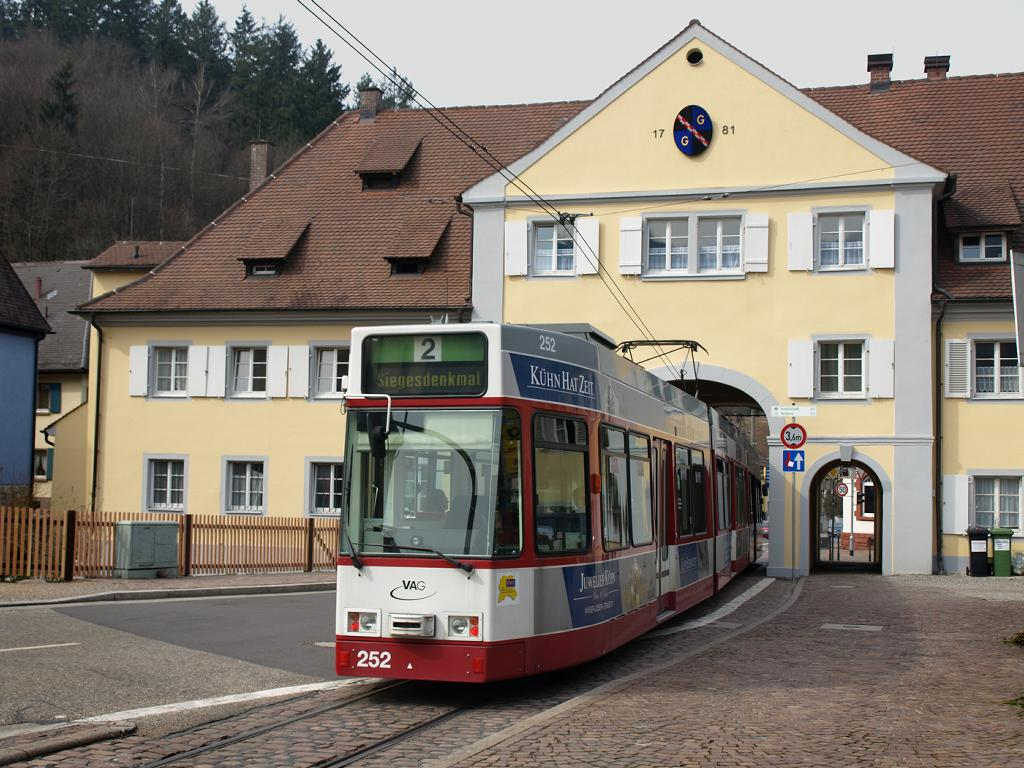
\includegraphics[width=\linewidth]{./figures/tor.png}
  \captionof{figure}{\iftoggle{isEnglish}{Gatehouse of the former monastery}{Torhaus des ehemaligen Klosters}}
	\setlength{\parskip}{0.25cm}

    \iftoggle{isEnglish}{
  Starting in 1926, he held an honorary professorship at the \alert{Albert-Ludwigs-Universität} in Freiburg im Breisgau, but had to give up this position in 1935 because he refused to begin his lectures with the Hitler salute, which was reported by colleagues (Gustav Doetsch and his assistant Eugen Schlotter). After the Second World War, he resumed his position as honorary professor, but due to his health condition, he was no longer able to give lectures.
}{
	Er arbeitete ab 1926 mit einer Ehren-Professur an der \alert{Albert-Ludwigs-Universität} in Freiburg im Breisgau, musste diese Arbeit aber 1935 wieder aufgeben, da er sich weigerte die Vorlesungen mit Hitlergruß zu beginnen, was von Kollegen (Gustav Doetsch und dessen Assistent Eugen Schlotter) denunziert wurde. Nach dem Zweiten Weltkrieg bezog er seine Position als Honorarprofessor wieder, konnte aber aufgrund seines gesundheitlichen Zustandes keine Vorlesungen mehr halten.
}

\end{minipage}%
\newpage
\begin{minipage}[t]{0.31\textwidth}
	\vspace{0cm}
	\setlength{\parskip}{0.25cm}

	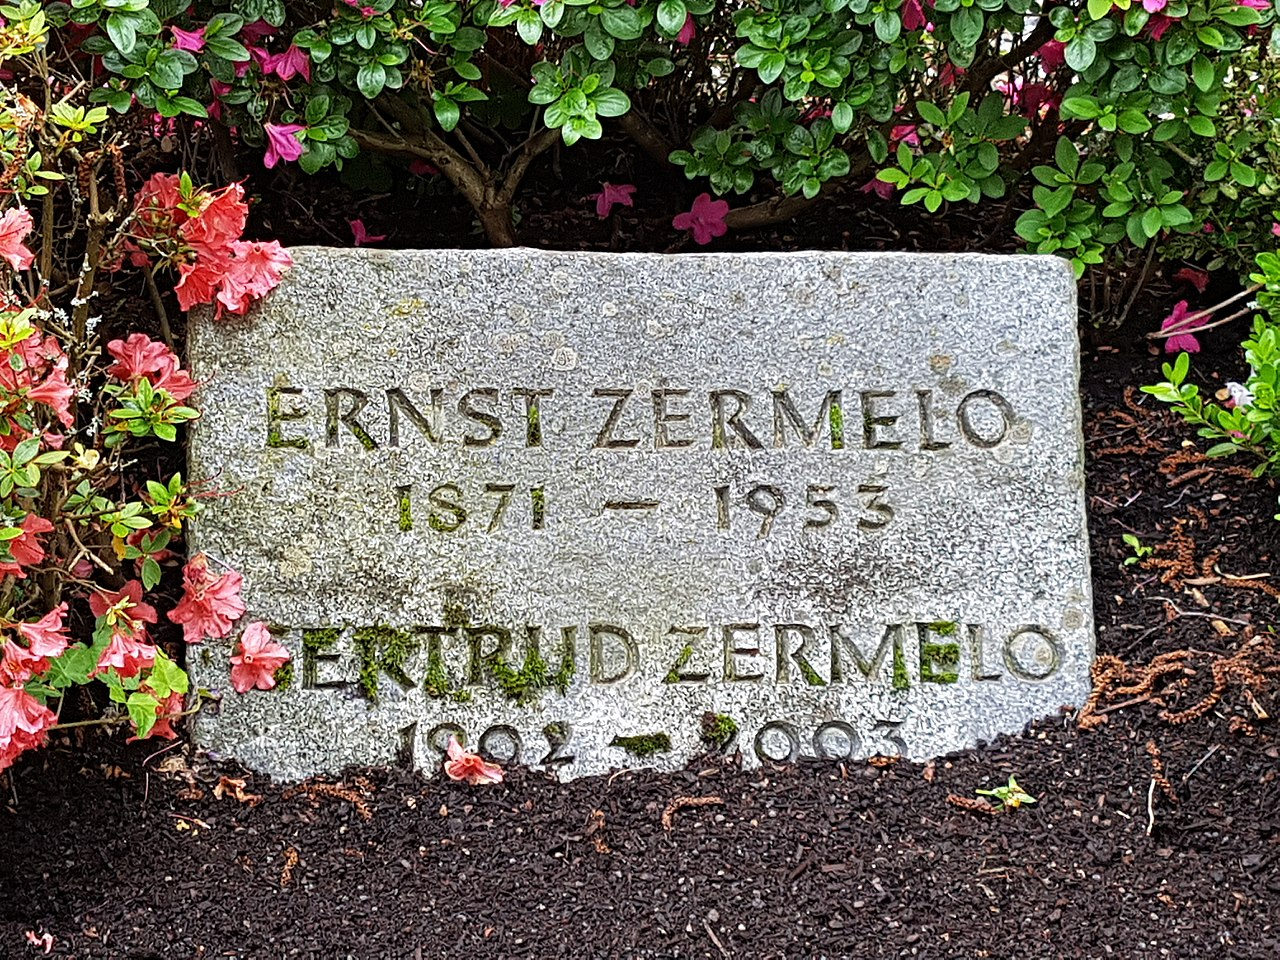
\includegraphics[width=\linewidth]{./figures/grabstein.png}
  \captionof{figure}{\iftoggle{isEnglish}{Gravestone of Ernst Zermelo in the Günterstal cemetery}{Grabstein von Ernst Zermelo im Friedhof Günterstal}}
	\setlength{\parskip}{0.25cm}

    \iftoggle{isEnglish}{
  In April 2018, the Eckerstraße in Freiburg, where the Mathematical Institute of the Albert-Ludwigs-Universität Freiburg is located, was renamed \alert{Ernst-Zermelo-Straße} in his honor. As the explanatory sign beneath the new name states, the street was renamed due to the problematic pioneering role of Alexander Ecker as a nationalist racial ideologist. The new name is well chosen for the institute: Ernst Zermelo is the namesake of the home address of the Ernst Mach Institute and the mathematics education department of the University of Freiburg, both are institutions that likely would not get far without Zermelo's set theory. % Even a celestial body, the asteroid 14990 Zermelo, is named after the mathematician.
}{
	Im April 2018 wurde in Freiburg ihm zu Ehren die Eckerstraße, in der sich das Mathematische Institut der Albert-Ludwigs-Universität Freiburg befindet, in \alert{Ernst-Zermelo-Straße} umbenannt. Wie das Erläuterungsschild unter dem neuen Namen erklärt, wurde die Straße aufgrund der problematischen Vorreiterrolle Alexander Eckers als völkischer Rassenideologe umbenannt. Der neue Name ist für das Institut gut ausgewählt: Ernst Zermelo ist Namensgeber der Heimatadresse des Ernst-Mach-Instituts und der Mathematikdidaktik der Universität Freiburg, beides sind Institutionen, die ohne die Zermelo’sche Mengenlehre der Mathematik wohl nicht weit kämen. % Sogar ein Himmelskörper, der Asteroid 14990 Zermelo, ist nach dem Mathematiker benannt.
}

	\includegraphics[width=\linewidth]{./figures/straßenschild.png}
  \captionof{figure}{\iftoggle{isEnglish}{Former Eckerstraße renamed to Ernst-Zermelo-Straße}{Ehemalige Eckerstraße in Ernst-Zermelo-Straße umbenannt}}
	\setlength{\parskip}{0.25cm}
\end{minipage}%
\hfill%
\vrule width 0.01cm
\hfill%
\begin{minipage}[t]{0.31\textwidth}
  \vspace{0cm}
	\setlength{\parskip}{0.25cm}

    \iftoggle{isEnglish}{
  Along the hiking route, you come to the \alert{Kybfelsen castle ruin}, which lies mysteriously hidden among the trees. A castle on the Kybfelsen is mentioned in the chronicle of Matthias of Neuenburg from the mid-14th century. The name \enquote{Kyburg} first appears in 1484 in the legal code of Kappel. Excavation findings at the castle site in the 1920s by Otto Kantorowicz confirm the existence of the structure already during the rule of the Zähringer dynasty in the Breisgau in the late 11th or early 12th century. % Finds of reading ceramics, which can be dated to the 12th and early 13th centuries, complete the picture of the period during which the fortified site was in use.

The \alert{district of Zähringen} in Freiburg is named after the Zähringer dynasty, a noble family that played a significant role in the region during the Middle Ages. The district name \enquote{Zähringen} is derived from the former Zähringen Castle, which was built in the 11th century by the Zähringer. This castle was located near today’s Zähringen district and served as a strategically important point to control the surrounding area. Zähringerstraße and Zähringen Castle still bear witness to this history.

The \alert{Zähringen Castle} on the Schlossberg lost its importance in the 13th century and was later destroyed. Today, only a few remnants of the castle remain. The ruins are located on the Zähringen Hill in the Zähringen district, where the foundations and parts of the former castle complex can still be seen.
}{
	Auf der Wanderroute geht es zur \alert{Burg Kybfelsen}, die geheimnisvoll zwischen den Bäumen verborgen liegt. Eine Burg auf dem Kybfelsen wird in der Chronik des Matthias von Neuenburg aus der Mitte des 14. Jahrhunderts erwähnt. Der Name \enquote{Kyburg} taucht erstmals 1484 im Weistum von Kappel auf. Erbrachtes Fundmaterial aus Grabungen an der Burgstelle in den 1920er Jahren durch Otto Kantorowicz belegen die Existenz der Anlage bereits während der Zeit der Zähringer Herrschaft im Breisgau des späten 11. bzw. frühen 12. Jahrhunderts. %Lesekeramikfunde, die sich in das 12. und frühe 13. Jahrhundert datieren lassen, vervollständigen die Sicht auf den Nutzungszeitraum des befestigten Platzes

	Der \alert{Stadtteil Zähringen} in Freiburg hat seinen Namen von der Zähringer Dynastie, einem Adelsgeschlecht, das im Mittelalter eine bedeutende Rolle in der Region spielte. Der Name \enquote{Zähringen} leitet sich von der ehemaligen Zähringer Burg ab, die im 11. Jahrhundert von den Zähringern erbaut wurde. Diese Burg lag in der Nähe des heutigen Zähringer Stadtteils und war ein strategisch wichtiger Punkt, um das Umland zu kontrollieren. Die Zähringerstraße und das Zähringer Schloss sind noch heute Zeugen dieser Geschichte.

	Die \alert{Zähringer Burg} auf dem Schlossberg verlor im 13. Jahrhundert an Bedeutung und wurde später zerstört. Heute sind nur noch wenige Reste der Burg erhalten. Die Überreste befinden sich auf dem Zähringer Berg im Stadtteil Zähringen, wo man noch die Grundmauern und Teile der ehemaligen Burganlage finden kann.
}

	\includegraphics[width=\linewidth]{./figures/kybfelsen.png}
  \captionof{figure}{\iftoggle{isEnglish}{The castle ruins of Kybfelsen}{Die Burgruine Kybfelsen}}
	\setlength{\parskip}{0.25cm}

    \iftoggle{isEnglish}{
  The \alert{Zähringer} were an important Swabian princely dynasty of the Middle Ages that played a decisive role in the founding and development of Freiburg im Breisgau. Duke Conrad of Zähringen founded the city in 1120 as a market town by establishing a market and allocating plots to merchants. The Zähringer built a castle on the Schlossberg in 1091, which significantly promoted the city's development. They granted Freiburg extensive freedoms and privileges, turning the city into the center of their dominion. These measures helped to advance trade and the economic development of the region. After the extinction of the Zähringer line in 1218, Freiburg passed to the Counts of Urach, who from then on called themselves Counts of Freiburg. Nevertheless, the positive memory of the Zähringer as founders and patrons of the city remained alive in Freiburg. Their legacy left a lasting mark on the development of the city and the entire region between the Black Forest and Lake Geneva.
}{
	Die \alert{Zähringer} waren ein bedeutendes schwäbisches Fürstengeschlecht des Mittelalters, das eine entscheidende Rolle bei der Gründung und Entwicklung von Freiburg im Breisgau spielte. Herzog Konrad von Zähringen gründete die Stadt im Jahr 1120 als Marktstadt, indem er einen Markt einrichtete und Kaufleuten Grundstücke zuwies. Die Zähringer bauten 1091 eine Burg auf dem Schlossberg, was die Stadtentwicklung maßgeblich förderte. Sie verliehen Freiburg weitreichende Freiheiten und Privilegien, wodurch die Stadt zum Zentrum ihres Herrschaftsgebiets wurde. Diese Maßnahmen trugen dazu bei den Handel und die wirtschaftliche Entwicklung der Region voranzutreiben. Nach dem Aussterben der Zähringer im Jahr 1218 ging Freiburg an die Grafen von Urach über, die sich fortan Grafen von Freiburg nannten. Dennoch blieb das positive Andenken an die Zähringer als Stadtgründer und Förderer in Freiburg erhalten. Ihr Erbe prägte nachhaltig die Entwicklung der Stadt und der gesamten Region zwischen Schwarzwald und Genfer See.
}

	% 1080 wurde in einem Bericht Otto von Freisings erstmals eine Burg Zähringen erwähnt, ein erster urkundlicher Nachweis befindet sich im Rotulus Sanpetrinus von 1128. Die Entstehungsgeschichte der Burg liegt im Dunkeln. Das darunterliegende Dorf Zähringen wurde 1008 erstmals in einer Schenkungsurkunde, der sogenannten Wildbannurkunde von König Heinrich II. an das Bistum Basel erwähnt, zusammen mit den Namen der Freiburger Stadtteile Herdern und Wiehre, der Nachbargemeinde Gundelfingen und anderer Orte im Breisgau.
\end{minipage}%
\hfill\color{white}%
\vrule width 0.01cm
\hfill\color{black}%
\begin{minipage}[t]{0.31\textwidth}
	\vspace{0cm}
	\setlength{\parskip}{0.25cm}

    \iftoggle{isEnglish}{
	% Ein kulinarischer Höhepunkt erwartet einen im \alert{Waldrestaurant St. Valentin}, wo regionale Spezialitäten und kühle Getränke zur Stärkung erworben werden können. \alert{St. Valentin} war ein christlicher Märtyrer aus dem 3. Jahrhundert, von dem es mehrere Überlieferungen gibt, darunter als ein Priester in Rom und ein Bischof in Terni. Er wird oft mit heimlichen Eheschließungen in Verbindung gebracht, was zu seiner späteren Hinrichtung führte. Die Assoziation mit dem Valentinstag und der Liebe entstand jedoch erst im Mittelalter und basiert mehr auf romantischen Traditionen als auf historischen Tatsachen.
  A culinary highlight awaits you at the \alert{forest restaurant St. Valentin}, where regional specialties and cool drinks can be enjoyed for refreshment. \alert{St. Valentin} was a Christian martyr from the 3rd century, about whom there are several accounts, including one as a priest in Rome and another as a bishop in Terni. He is often associated with performing secret marriages, which ultimately led to his execution. However, the association with Valentine's Day and love only emerged in the Middle Ages and is based more on romantic traditions than on historical facts.
}{
	Ein kulinarischer Höhepunkt erwartet einen im \alert{Waldrestaurant St. Valentin}, wo regionale Spezialitäten und kühle Getränke zur Stärkung erworben werden können. \alert{St. Valentin} war ein christlicher Märtyrer aus dem 3. Jahrhundert, von dem es mehrere Überlieferungen gibt, darunter als ein Priester in Rom und ein Bischof in Terni. Er wird oft mit heimlichen Eheschließungen in Verbindung gebracht, was zu seiner späteren Hinrichtung führte. Die Assoziation mit dem Valentinstag und der Liebe entstand jedoch erst im Mittelalter und basiert mehr auf romantischen Traditionen als auf historischen Tatsachen.
}

	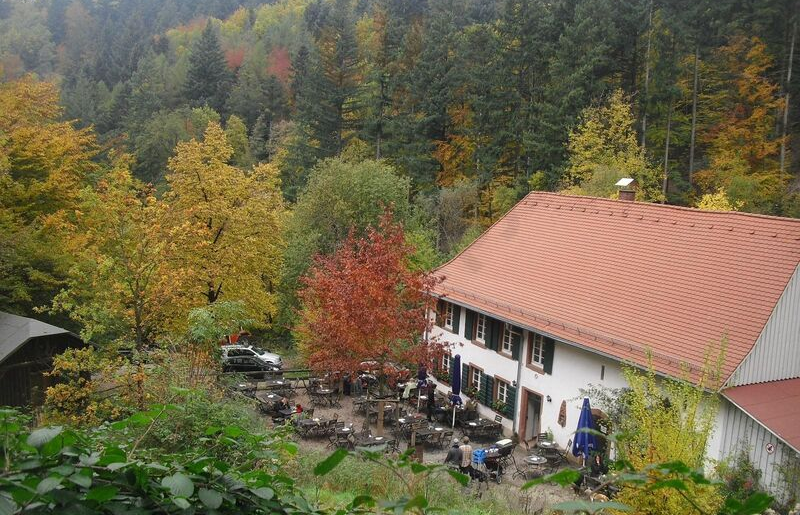
\includegraphics[width=\linewidth]{./figures/stvalentin_2.png}
  \captionof{figure}{\iftoggle{isEnglish}{Forest restaurant St. Valentin from a bird’s-eye view}{Waldrestaurant St. Valentin aus der Vogelperspektive}}
	\setlength{\parskip}{0.25cm}


    \iftoggle{isEnglish}{
  % Echoing the legacy of Roman architectural influence, the \alert{St. Lioba Monastery} in Freiburg Günterstal is housed in a Tuscan-style villa that was established in 1927. Tuscan style is a classical architectural tradition from central Italy, rooted in Roman and Renaissance design, featuring symmetry, earthy materials, and terracotta. Terracotta is a type of baked clay that’s been used for thousands of years in art, architecture, and construction. \alert{St. Lioba} (c. 710–782) was an English nun and missionary. She helped spread Christianity in what is now Germany.
  At the end of our journey, we arrive at the \alert{St. Lioba Monastery}, nestled in a Tuscan-style villa established in 1927. This architectural style, originating in central Italy, it reflects classical Roman and Renaissance influences with its balanced symmetry, earthy materials, and signature terracotta elements (baked clay that has been used for millennia in art and construction). The monastery is named after St. Lioba (c. 710–782), an English nun and missionary who played a key role in spreading Christianity in what is now Germany
}{
  Am Ende unserer Reise ereichen wir das Das \alert{St. Lioba-Kloster}, welches sich sich in einer Villa im toskanischen Stil, erbaut 1927 befindet. Dies ist eine Anlehnung an römisch-renaissancistische Architektur mit Symmetrie, Naturmaterialien und Terrakotta. Terrakotta ist ein gebrannter Ton, der seit Jahrtausenden im Bauwesen verwendet wird. \alert{St. Lioba} (ca. 710–782) war eine englische Nonne und Missionarin, die zur Christianisierung im heutigen Deutschland beitrug.
}

  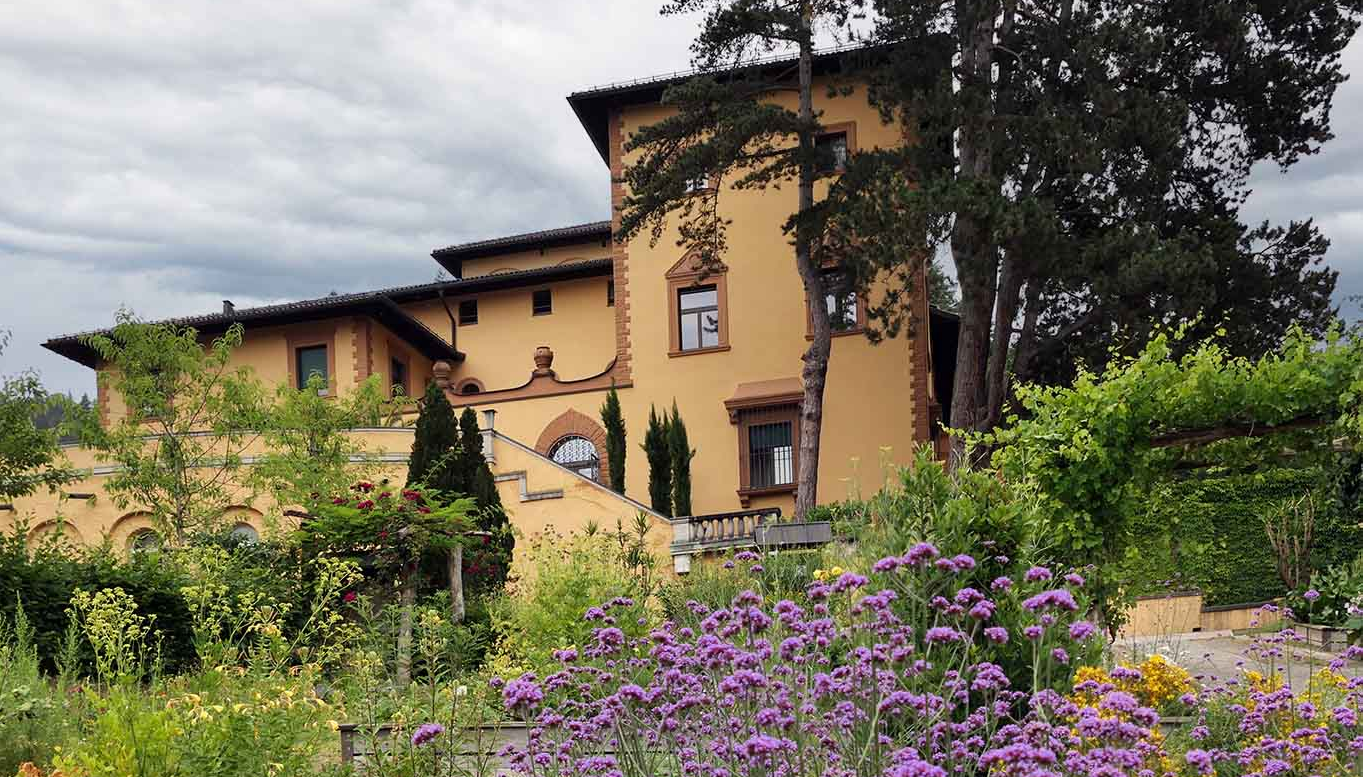
\includegraphics[width=\linewidth]{./figures/kloster_st_lioba.png}
  \captionof{figure}{\iftoggle{isEnglish}{St. Lioba Monastery, where Roman architecture lives on}{Kloster St. Lioba, wo römische Architektur weiterlebt}}
	\setlength{\parskip}{0.25cm}

\end{minipage}%
\newpage
\begin{minipage}[t]{0.31\textwidth}
	\setlength{\parskip}{0.25cm}

	\vspace{0.5cm}

		\textcolor{PrimaryColor}{
			\rule{\linewidth}{0.5mm}
			\vspace{-0.1cm}
			\begin{center}
				\large
				\textsc{Addendum}
			\end{center}
			\rule{\linewidth}{0.5mm}
		}

    \iftoggle{isEnglish}{
  The Freiburg district of \alert{St. Georgen} by the way owes its name to another Christian saint, Saint George. The name most likely derives from an early chapel or church that was dedicated to Saint George, as this saint was considered an important patron in the Middle Ages. Saint George was a Roman soldier and martyr of the 3rd century who died for his Christian faith. According to legend, he slew a dragon and thus saved a city, with the dragon legend symbolizing his role as a defender of good and of the Christian faith. As a patron saint of many countries and professions, especially knights and soldiers, he stands for courage, steadfastness, and commitment to faith.

It’s a curious link between past and present that the district \alert{Vauban}, today a symbol of sustainable living, is named after a military engineer who once fortified Freiburg centuries ago. The name Vauban refers to \alert{Sébastien Le Prestre de Vauban} (1633–1707), a famous French military engineer who served under King Louis XIV. He was renowned for his innovative fortifications and siege tactics across Europe. During the 17th century, when France temporarily occupied parts of what is now southwestern Germany (including Freiburg), Vauban was involved in strengthening fortifications in the region. In fact, Freiburg's old city fortifications were redesigned under his influence during the French occupation (especially during 1677–1687). Fast forward to the late 20th century, in the 1990s, Freiburg began transforming an old French military base (used by the French army after WWII) into an eco-friendly, sustainable urban district. That area was named Vauban, in reference to the historical military presence and French influence. 
}{
	Der Freiburger Stadtteil \alert{St. Georgen} hat seinen Namen einem anderen christlichen Heiligen, dem heiligen Georg zu verdanken. Der Name leitet sich höchstwahrscheinlich von einer frühen Kapelle oder Kirche ab, die dem heiligen Georg geweiht war, da dieser Heilige im Mittelalter als wichtiger Schutzpatron galt. Es war damals üblich, Siedlungen nach Heiligen zu benennen, die als Schutzpatrone für die Region fungierten und die Sicherheit und den Segen Gottes für die Gemeinschaft repräsentierten.

	Der \alert{heilige Georg} war ein römischer Soldat und Märtyrer des 3. Jahrhunderts, der für seinen christlichen Glauben starb. Georg wurde aufgrund seines christlichen Glaubens verfolgt und schließlich während der Diokletianischen Christenverfolgung (ca. 303 n. Chr.) in Lydda (im heutigen Israel) als Märtyrer getötet. Da er sich weigerte, den christlichen Glauben aufzugeben und dem römischen Götterkult zu opfern, wurde er gefoltert und schließlich geköpft. Die Legende besagt, er habe einen Drachen besiegt und dadurch eine Stadt gerettet, wobei die Drachenlegende seine Rolle als Verteidiger des Guten und des christlichen Glaubens symbolisiert. Als Schutzpatron vieler Länder und Berufe, besonders der Ritter und Soldaten, steht er für Mut, Standhaftigkeit und den Einsatz für den Glauben.

  Es ist eine interessante Verbindung zwischen Vergangenheit und Gegenwart, dass der Stadteil \alert{Vauban}, heute ein Symbol für nachhaltiges Leben, nach einem Militäringenieur benannt ist, der Freiburg vor Jahrhunderten befestigte. Der Name Vauban bezieht sich auf \alert{Sébastien Le Prestre de Vauban} (1633–1707), einen berühmten französischen Militäringenieur, der unter König Ludwig XIV. diente. Er war bekannt für seine innovativen Befestigungen und Belagerungstaktiken in ganz Europa. Im 17. Jahrhundert, als Frankreich zeitweise Teile des heutigen Südwestdeutschlands (einschließlich Freiburg) besetzte, war Vauban an der Verstärkung der Befestigungsanlagen in der Region beteiligt. Tatsächlich wurden Freiburgs alte Stadtbefestigungen während der französischen Besatzung (insbesondere zwischen 1677 und 1687) unter seinem Einfluss umgestaltet. In den 1990er Jahren, also Jahrhunderte später, begann Freiburg damit, eine ehemalige französische Militärbasis (die nach dem Zweiten Weltkrieg von der französischen Armee genutzt wurde) in ein umweltfreundliches, nachhaltiges Stadtviertel umzuwandeln. Dieses Gebiet wurde Vauban genannt, als Verweis auf die historische militärische Präsenz und den französischen Einfluss. 
}
\end{minipage}%

  %At that time, it was common to name settlements after saints who served as patrons for the region and represented God's protection and blessing for the community.
%   The Freiburg district of \alert{St. Georgen} owes its name, by the way, to another Christian saint, Saint George. The name most likely derives from an early chapel or church that was dedicated to Saint George, as this saint was considered an important patron in the Middle Ages. At that time, it was common to name settlements after saints who served as patrons for the region and represented God's protection and blessing for the community.
%
% \alert{Saint George} was a Roman soldier and martyr of the 3rd century who died for his Christian faith. George was persecuted because of his Christian beliefs and was eventually martyred during the Diocletianic Persecution (around 303 AD) in Lydda (in present-day Israel). Because he refused to renounce his Christian faith and make sacrifices to the Roman gods, he was tortured and eventually beheaded. According to legend, he slew a dragon and thus saved a city, with the dragon legend symbolizing his role as a defender of good and of the Christian faith. As a patron saint of many countries and professions, especially knights and soldiers, he stands for courage, steadfastness, and commitment to faith.

\end{document}
